%%%%%%%%%%%%%%%%%%%%%%%%%%%%%%%%%%%%%%%%%%%%%
\section{\dinv design}
\label{sec:instrumentation}
%%%%%%%%%%%%%%%%%%%%%%%%%%%%%%%%%%%%%%%%%%%%%

Applying \dinv to a system consists of four steps
(Figure~\ref{fig:dinv-flow}): (1) source code instrumentation, (2) system
execution to generate runtime logs, (3) mining of distributed program
states from the logs, and (4) determining likely distributed state
invariants from distributed program points. This section details each
of these steps.

%%%%%%%%%%%%%%%%%%%%%%%%%%%%%%%%%%%%%%%%%%%%%%%%%%%%%%%%%%%%%%%%%%%%%%
\begin{figure*}[t]
\centering
    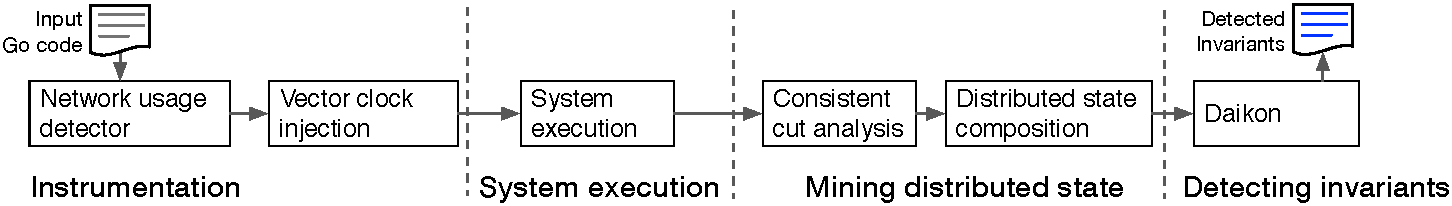
\includegraphics[width=.9\textwidth]{fig/dinv-flow.pdf}
    \caption{Overview of the steps in \dinv.}
    \label{fig:dinv-flow}
\end{figure*}

%%%%%%%%%%%%%%%%%%%%%%%%%%%%%%%%%%%%%%%%%%%%%
\subsection{System instrumentation}
\label{sec:instrumentation}
%%%%%%%%%%%%%%%%%%%%%%%%%%%%%%%%%%%%%%%%%%%%%

\dinv instruments a node's source code to produce a runtime log
containing vector-timestamped node state (each process maintains its
own vector clock).
%%   when the
%% instrumented program is executed. A log requires vector timestamps to
%% establish a partial ordering, and the values of variables defining the
%% nodes state.
Maintaining vector clocks (see Appendix~\ref{sec:formal-vector-clocks}
for the algorithm) and logging of variables require separate forms of
instrumentation.  We developed automated techniques for both.

% JS: awkward enumeration. Why not just: Protocol-handling code in
% \textit{net} remains unmodified, except for RPC share function
% signatures, which are wrapped by Dinv:...
% ... to interpose on RPC, we have built a custom codec.

\textbf{Injecting vector clocks.}
Dinv introduces vector clocks automatically by mutating the AST and by
exploiting the conventions followed by Go's networking \textit{net}
library. This library implements TCP, IP, UDP, RPC, and IPC protocols;
all of these, except for RPC, share function signature conventions which
Dinv wraps:
%% Dinv injects a custom wrapper function, and pass the original
%% function, and its arguments into the wrapper.  Within a wrapper
%% function,
vector clocks are appended or stripped from network payloads, and the
original function is executed on the instrumented arguments. For
example, a network write like \texttt{conn.Write(buffer)} becomes
\texttt{dinv.Write(conn.Write,buffer)}.  For Go's RPC, which required
a different approach, we built a custom codec. By using these two
techniques \dinv adds vector clocks to any Go program that uses the
\textit{net} library.

%%  in the background. Initializing an RPC
%% connection requires calls to the standard RPC library.
%
%% The same function capturing technique which injects vector clocks is used on
%% such calls to automatically inject the vector clock codec.
%

%%%%%%%%%%%%%%%%%%%%%%%%%
%\subsection{Logging state}
%%%%%%%%%%%%%%%%%%%%%%%%%

%%%%%%%%%%%%%%%%%%%%%%%%%%%%%%%%%%%%%%%%%%%%%
\begin{figure}[t]
    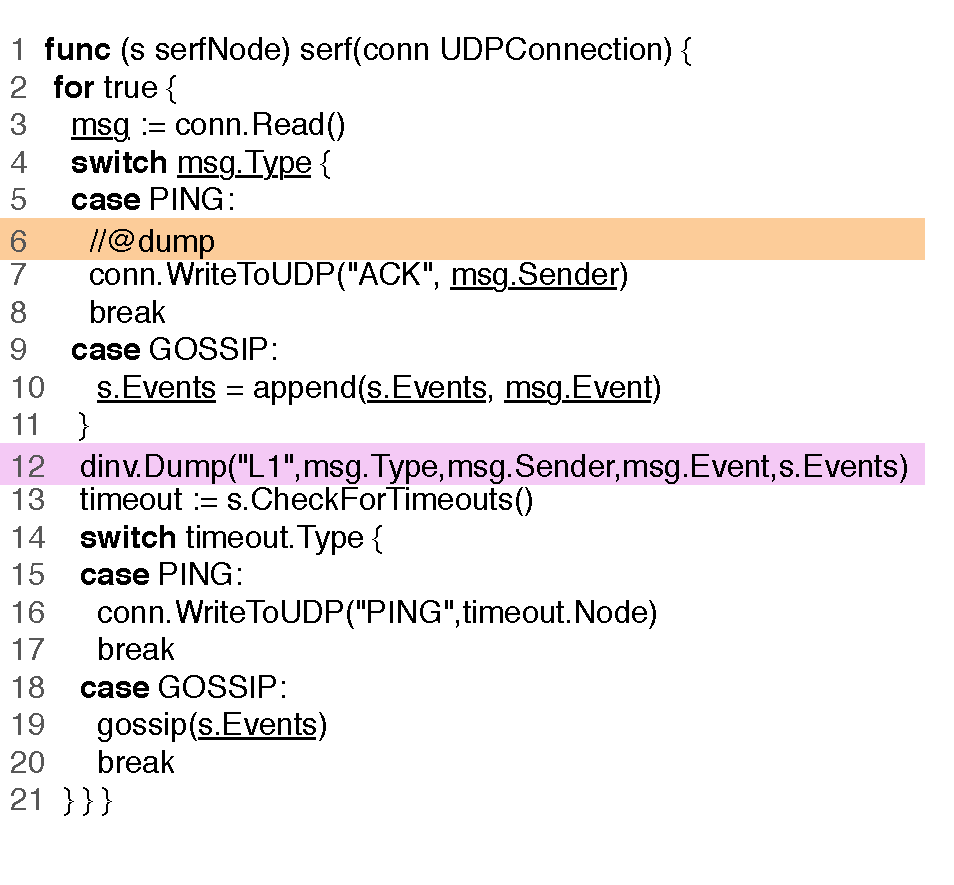
\includegraphics[width=0.50\textwidth]{fig/data-flow-3}
    \caption{Example illustrating network interacting variables
      (underlined) contained in the forward slice from $msg :=
      conn.Read()$. Two annotations on lines 6 and 12 are also
      highlighted.
      %% A dump annotation is highlighted in
      %% orange. Highlighted in magenta is logging code translated from
      %% an annotation containing networking variables.
    }
  \label{fig:data-flow}
\end{figure}
%%%%%%%%%%%%%%%%%%%%%%%%%%%%%%%%%%%%%%%%%%%%%

\textbf{Logging node state.} We designed Dinv with the assumption that
interesting state in a distributed system is composed of variables
which interact with the network. Data read from a network transitively
affects variables which interact with it, while variables which affect
the contents of network writes have a transitive influence on the
behaviour of the node that receives the message. These \emph{network
  interacting variables} influence the state of other nodes, and
properties that range over these variables capture information about
the consistency of distributed state. Dinv determines the network
interacting variables statically using interprocedural program
slicing~\cite{Ottenstein:1984, Walkinshaw03thejava}. It provides
developers with three options (Table~\ref{table:inst-strat}): (1)
automatically log these variables at all function enter/exit points,
(2) automatically log these variables at developer-annotated points,
or (3) log variables interesting to the developer at
developer-annotated points.

Dinv also allows the developer to choose between two strategies for
recording state: {\tt dump} records values at the dump statement
program point, while {\tt track} delays recording of values until
just before a network communication event. That is, track statements
aggregate state across different program scopes for a more complete
view, but they are not as precise as dump statements.

%% At each event instance a node has a distinct state and each
%% instruction that it executes potentially modifies this state.
%% %% Capturing state is an essential component of recording a log. 
%% %% , as such a complete log would contain the values of all variables
%% %% recorded after the execution of each instruction.
%% In practice, recording at this granularity is unmanageable.  Dinv
%% instead logs a subset of variables and logs these at select times.

Figure~\ref{fig:data-flow} lists partial code from Serf~\cite{serf}
that implements the SWIM protocol~\cite{das2002swim}. We will use this
example throughout the paper.
This code has two logging points in the form of {\tt //@dump}
annotation (line 6) and a \emph{paramatrized Dump} statement
(line 12). The first logs state when a \emph{Ping} is received, the
other logs state before checking for timeouts. The code also
illustrates the variables affected by a network read (underlined).
%
%% Both statements log variables within the
%% received message and the events stored on the Serf node.

%% The red highlighted variables are detected automatically through
%% static analysis by \dinv's instrumentation described in
%% Section~\ref{sec:logging-variables}, and will be logged by the
%% \emph{//@dump} annotation post instrumentation.

%% Some variables are resigned solely to local computation, and do not
%% interact with the network.  Testing invariants of such variables on
%% separate nodes would yield arbitrary results. To derive meaningful
%% distributed invariants we partition these sets of variables and
%% only log \emph{network interacting variables}, which can be
%% detected statically using program slicing~\cite{Ottenstein:1984}.
 
%%%%%%%%%%%%%%%%%%%%%%%%%%%%%%%%%%%%%%%%%%%%%
\begin{table}[t]
\centering
\small
%    \begin{tabular}{| p{2.0cm} | p{1.0cm} | p{1.0cm} |}
\begin{tabular}{ l  l  l }
\midrule
  Instrumentation strategy & \pbox{1.2cm}{Location choice} & \pbox{1.2cm}{Variables choice} \\ 
\midrule
  Entrance and exit of functions  &   Auto   & Auto \\
  User placed annotations   & Manual  & Auto \\ 
  Paramatrized logging functions & Manual & Manual \\ 
  \bottomrule
\end{tabular}
\caption{Instrumentation strategies and the control (automatic/manual)
  offered by each strategy for selecting state logging location and
  set of logged variables.}
\label{table:inst-strat}
\end{table}
%%%%%%%%%%%%%%%%%%%%%%%%%%%%%%%%%%%%%%%%%%%%%

%
% JS: Consider cutting this paragraph out for space.
%
The remainder of this section explains how the runtime node logs are
merged together, how the states of independent nodes are combined into
distributed program points, and how Dinv infers distributed data
invariants from these combined states.


%% In this section we outlined the two step procedure by which  \dinv
%% instruments a programs source code to produce a log. \dinv
%% automatically wraps network communication in order to maintain a
%% vector clock with the other nodes in the system.  Secondly, variable
%% logging statements are added using any configuration of the automated,
%% semi-automated, or manual dumping methods. In
%% Section~\ref{sec:log-analysis} we describe how the log is processed.
